\documentclass{article}

\usepackage{amsmath, tikz}
\usetikzlibrary{automata, positioning, arrows} 
\begin{document}
\textbf{Exercise 1}. In this exercise, we work over the alphabet $\Sigma$ = $\{a, b\}$. Show
that $L = \{a^nb^m \mid n > m \geq 0 \}$ is a context-free language. In other words,
exhibit a context-free grammar that generates $L$ and give a quick justification. \\

\textbf{ANSWER}:

The grammar exhibited is as follows: $G = (\Sigma, \{S, V\}, S, P)$, where $\Sigma$ is given, $S$ and $V$ are symbols, $S$ is the starting symbols, and $P$ is as follows:

\[S \rightarrow aV, \; V \rightarrow SV, \; V \rightarrow aSb, \; S \rightarrow a, \; S \rightarrow \varepsilon, \; V \rightarrow \varepsilon\]

The reason this CFG generates $L(\mathcal{A})$ is because any instance of $b$ must be met with an instance of $a$. Additionally, an infinite amount of $a$'s can be created by repeating the first two rules. $S \rightarrow a$ is an unnecessary rule (since the first and last rules can be used to make the fourth rule) but exists to make runs cleaner. As for edge cases, a singular $a$ can be made with the fourth rule, and an an infinite string of $a$'s can be made with the first, second, fourth, and sixth rules.\\

\textbf{Exercise 2}. In this exercise, we work over the alphabet $\Sigma = \{a, b\}$:

(i) Determine the language $L(G)$ generated by the grammar $G = (\Sigma, \{S\}, S, P)$
where $P$ contains the following production rules:
\[S \rightarrow \varepsilon_1, \; S \rightarrow a_2, \; S \rightarrow b_3, \; S \rightarrow c_4\]
\[S \rightarrow aSa_5, \; S \rightarrow bSb_6, \; S \rightarrow cSc_7\]

(ii) Choose a word of length at least 6 in the language you found and give
a derivation for it from $S$ in $G$. (We expect an answer in the form of a
sequence $S \Rightarrow \ldots \Rightarrow w$ where $w$ is the word you chose.)

\textbf{ANSWER}:

The language determined by $L(G)$ is the language of all palindromes over $a, b, c$. This is because for each instance of S, we either mirror a letter, or remove S and finalize our middle letter. If this letter is $\varepsilon$, we have a directly mirrored palindrome, and if its one of the letters in $\Sigma$, we have a palindrome thats mirrored around a letter (i.e., abbabba vs abba). 

Let's create a run for $abcacba$.

\[S\overset{5}\Rightarrow aSa, \; S\overset{6}\Rightarrow abSba, \;  S\overset{7}\Rightarrow abcScba, \;  S\overset{2}\Rightarrow abcacba\]

Where the numbers above the arrows correspond to the numbered rules. \\

\textbf{Exercise 3}. In this exercise, we work over the alphabet $\Sigma = \{a, b, c\}$. Con-
struct a PDA $\mathcal{A}$ over $\Sigma$ that recognizes the language $L$ of all palindromes.\\

\textbf{ANSWER}:

A clarification about the notation used in the construction of this PDA. When I write, for example $(l \in \{a, b, c\}, z \in \{0, 1, 2\}, zz \in \{0, 1, 2\})$, I intend this: a corresponds to 0, b corresponds to 1, and c coressponds to 2. This means that when you say $a$, you pop $0$, and push $00$, or when you say $b$, you pop $1$, and push $11$, etc. In all honesty, this is because I don't know how to angle loops in tikz. If you have questions please send me an email and I will respond asap. (By the way, $\Gamma = \{0, 1, 2\}$)
\begin{center}
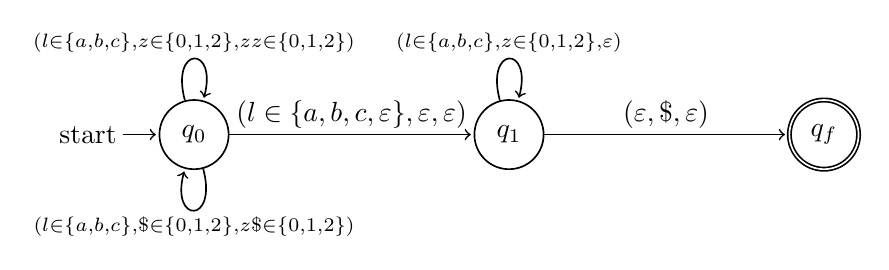
\begin{tikzpicture}
[->,shorten >=1pt,
                    auto,node distance=4cm,on grid,semithick,
                    inner sep=2pt,bend angle=45]

\node[state, initial] (q0) {$q_0$};
\node[state, right of=q0] (q1) {$q_1$};
\node[state, accepting, right of=q1] (qf) {$q_f$};

\path[->]
	(q0) edge [loop above] node {$\scriptstyle(l \in \{a, b, c\}, z \in \{0, 1, 2\}, zz \in \{0, 1, 2\})$} ()
		edge [loop below] node {$\scriptstyle(l \in \{a, b, c\}, \$ \in \{0, 1, 2\}, z\$ \in \{0, 1, 2\})$} ()
		edge node  {$(l \in \{a, b, c, \varepsilon\}, \varepsilon, \varepsilon)$} (q1)
	(q1) edge [loop above] node {$\scriptstyle(l \in \{a, b, c\}, z \in \{0, 1, 2\}, \varepsilon)$} ()
		edge node  {$(\varepsilon, \$, \varepsilon)$} (qf);
\end{tikzpicture}
\end{center}

\textbf{Exercise 4}. In this exercise, we work over the alphabet $\Sigma = \{a, b, c\}$ Con-
sider the following PDA $\mathcal{A}$ over $\Sigma$ and $\Gamma = {0, 1, \$}$: (its the one you gave us :D)

(i) Give $\mathcal{A}$ formally, by describing each of its seven components: $(\Sigma, \Gamma, Q, \delta, q_0, z, F)$.

(ii) Give a sequence of moves that shows that the word abbcbba is recognized\\
by $\mathcal{A}$

(iii) Determine the language $L(\mathcal{A})$.\\

\textbf{ANSWER}:

(i)
$\mathcal{A} := (\Sigma, \Gamma, Q, \delta, q_0, z, F)$ where $\Sigma = \{a, b, c\}$, $\Gamma = \{\$, x, 0, 1\}$, $Q = \{q_0, q_1, q_2, q_f\}$, $\delta$, $q_0 = q_0$, $z = \$$, $F = q_f$, where $\delta$ is defined by:
\begin{center}
$\delta(q_0, \varepsilon, \$) = \{q_1, \$\}$, (1)\\
$\delta(q_1, a, x) = \{q_1, 0x\}$, (2) \\
$\delta(q_1, b, x) = \{q_1, 1x\}$, (3)\\ 
$\delta(q_1, c, x )= \{q_2, x\}$, (4)\\ 
$\delta(q_2, a, 0) = \{q_2, \varepsilon\}$, (5)\\  
$\delta(q_2, b, 1) = \{q_2, \varepsilon\}$, (6)\\
$\delta(q_2, \varepsilon, \$) = \{q_f, \varepsilon\}$ (7)
\end{center}
(ii)
I took the liberty of labeling the transition relations in the previous step. Therefore, a sequence of moves that would recognize $abbcbba$ is simply: \[1 \rightarrow 2 \rightarrow 3 \rightarrow 3 \rightarrow 4 \rightarrow 6 \rightarrow 6 \rightarrow 5 \rightarrow 7\]

Which I will describe below:

Move from $q_0$ to $q_1$. At $q_1$, we say "$a, b, b$", which entails adding 100 to our stack. Then, we use the middle transition relation to add $c$ to our word. Then, we pop $100$ from the stack, saying $b, b, a$, and finally use the final transition relation to go to the final state, using the intial stack character.\\

(iii)
The language recognized by this PDA is the set of all palindromes over $\Sigma$ that have a $c$ in the middle. More formally, 
\[L(\mathcal{A}) = \{w c w^R \mid w \in \{a, b\}^*\} \]

And where $w^R$ entails the reversed form of $w$.

\textbf{Exercise 5 (Bonus)}. Prove rigorously your answer of (iii) in the previous exercise.

\textbf{ANSWER}:

To show that $L(\mathcal{A}) = \{w c w^R \mid w \in \{a, b\}^*\}$, we exhibit a run for $\mathcal{A}$, and show it is naturally of the form $wcw^R$. 

Let $(q_0, q_1, \ldots, q_f)$ be a successful run over $\mathcal{A}$, and call it $r$. This means we have a set of states that starts at $q_0$, and ends in $q_f$. This means that we must apply the following three transition relations in $\mathcal{A}$ in order to reach $q_f$:

\begin{center}
$\delta(q_0, \varepsilon, \$) = \{q_1, \$\}$, \\
$\delta(q_1, c, x )= \{q_2, x\}$,\\ 
$\delta(q_2, \varepsilon, \$) = \{q_f, \varepsilon\}$
\end{center}

Taking these three tranistions alone leaves us with the word $c$, which is of the form $wcw^R$, because since $w \in \{a, b\}^*$, $w$ can be equal to $\varepsilon$. 

We can then split $r$ into two sections. One of these sections,  $r_1 = (q_0, q_1, \ldots, q_i)$, is the set of states before the transition $\delta(q_1, c, x )= \{q_2, x\}$, and the other section, $r_2 = (q_i+1, \ldots, q_f)$ is the section after the transition. For any transition we take in $r_1$, we push a series of characters, $z_1$, onto the stack. In $r_2$, we must continually pop these characters off of the stack until we are left with $\$$, which then allows us to take the transition $\delta(q_2, \varepsilon, \$) = \{q_f, \varepsilon\}$, and allows our run to be successful. Because of the nature of the stack, the first character we pushed onto the stack becomes the last character we pop off of the stack, and vice versa. We know that any instance of $1$ on the stack corresponds to a $b$ in our word, and similarly any $0$ on the stack corresponds to an $a$ in our word. In order for our run to be successful, we must pop all symbols besides $\$$ off of the stack, so that we can take the transition $\delta(q_2, \varepsilon, \$) = \{q_f, \varepsilon\}$ to reach $q_f$.  That means we have a word $w$, which corresponds to the stack symbol $z_1$, and by popping each symbol in $z_1$ off of the stack in the opposite order that they were pushed, we say the corresponding letter in $w$ in reverse. Hence, we must say $wcw^R$, as desired.
\end{document}
